\section{The MNIST Dataset}
\vspace{1cm}
The MNIST (Modified National Institute of Standards and Technology) dataset \cite{lecun1998} is a large collection of handwritten digits commonly used for training various image processing systems. It serves as a benchmark for evaluating the performance of machine learning algorithms. The dataset contains 60,000 training images and 10,000 test images, each of which is a gray scale image of size \( 28 \times 28 \) pixels.
\\\\
Each image in the MNIST dataset is labeled with the digit it represents, ranging from 0 to 9. The dataset is particularly valuable because it provides a diverse set of handwriting styles, allowing for the development of robust digit recognition systems.

\begin{itemize}
    \item \textbf{Size:} The training set consists of 60,000 images, and the test set consists of 10,000 images.
    \item \textbf{Resolution:} Each image is \( 28 \times 28 \) pixels, making a total of 784 features.
    \item \textbf{Classes:} There are 10 classes, corresponding to the digits 0 through 9.
    \item \textbf{Grayscale:} Images are in grayscale, with pixel values ranging from 0 (black) to 255 (white).
\end{itemize}

\begin{figure}[h]
    \centering
    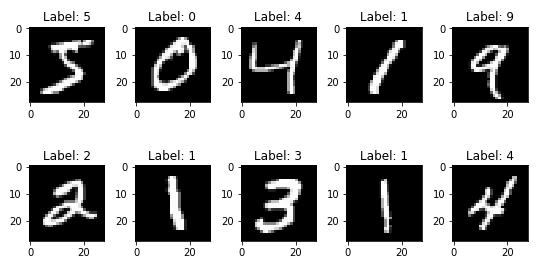
\includegraphics[width=0.7\textwidth]{assets/MNIST.png}
    \caption{Sample of images from the MNIST dataset}
    \label{fig:MNIST samples}
\end{figure}

